%===============================================================
% Universidade Tecnológica Federal do Paraná
% Departamento Acadêmico de Eletrônica
% Departamento Acadêmico de Informática
% Engenharia de Computação
% Oficina de Integração 3 (IF66J)
% Modelo e instruções para a elaboração dos
% relatórios técnicos da disciplina IF66J
% Autores: Gustavo B. Borba e Guilherme A. Schneider
% Versão: 05.abr.2015
%===============================================================

% Preâmbulo

% http://easylatek.blogs.sapo.pt/3034.html [---
\documentclass[a4paper,11pt]{article}
\usepackage[portuguese]{babel}
% Para Windows
\usepackage[utf8]{inputenc} %substituir 'latin1' por 'utf8' para editores ShareLaTex ou Overleaf
\usepackage[T1]{fontenc}
% Para Linux
% \usepackage[utf8]{inputenc}
% Para Mac
% \usepackage[applemac]{inputenc}
% ---]
% Packages [---
\usepackage{fancyhdr} %para copeçalho e rodapé
\usepackage{fancybox} %para copeçalho e rodapé
\pagestyle{fancy} %para copeçalho e rodapé
\usepackage{easylist} %para aninhar enumerate
\usepackage{paralist} %para compactenum
\usepackage{pbox} %para parbox
\usepackage[hyphens]{url}  %para url com line break
\usepackage{multirow} %para multirow e multicolumn
\usepackage{array, hhline} %mais opcoes para o ambiente tabular
\usepackage{fourier} %symbols
\usepackage{ifsym} %symbols
\usepackage{graphicx} %para inserir jpg e png e pdf
\usepackage{float}
\usepackage{pdfpages}
% ---]

% Cria hyperlinks e estrutura de tópicos para navegar em um pdf reader [---
% Não alterar
\usepackage{hyperref}
\usepackage{color}
\definecolor{corlinkprint}{rgb}{0, 0, 0}
\hypersetup{
  colorlinks,
  citecolor   = corlinkprint,
  filecolor   = corlinkprint,
  linkcolor   = corlinkprint,
  urlcolor    = corlinkprint}
% ---]

% Cabeçalho e rodapé a partir da página 2 [---
% Substituir 'Modelo' pelo nome do projeto (nome de uma palavra usado na disciplina)
\fancyhead[L]{\small{Relatório Técnico: Wall-e}}
\fancyhead[R]{\small\thepage} 
\fancyfoot{}
\renewcommand\headrulewidth{0.4pt}
% ---]

% Título [---
% Substituir 'Modelo...' pelo título do relatório
\title{
Relatório Técnico\\
\textbf{Wall-e: navegação autônoma baseada em mapas de custo, teleoperação e mapeamento 3D.}}
% ---]

% Autores [---
% Substituir pelos nomes e emails dos integrantes
\author{
Felipe Ukan Pereira \footnotesize{-- felipe.ukan@gmail.com}\\
Hudo Cim Assenço \footnotesize{-- hudo.assenco@gmail.com}\\
Rodrigo Longui Guimarães \footnotesize{-- rolongui@yahoo.com.br}\\
André Lucas Zanellato \footnotesize{-- andre.zanellato@gmail.com}\\
}
% ---]

% Substituir pelo mes e ano da defesa [---
\date{julho de 2015}
% ---]

\begin{document}

% Cabeçalho da página 1 [---
% Não alterar
\thisfancyput(35mm,-10mm){
\begin{tabular}{c}
Universidade Tecnológica Federal do Paraná -- \small{UTFPR}\\
Departamento Acadêmico de Eletrônica -- \small{DAELN}\\
Departamento Acadêmico de Informática -- \small{DAINF}\\
Engenharia de Computação\\
Oficina de Integração 3 (IF66J) -- S71 -- 2015/1 \\
\\
\hline
\end{tabular}}
% ---]

% Insere título, autores e data [---
\maketitle
% ---]

% Resumo [---
% Sustituir pelo seu resumo
\begin{abstract}
\noindent Este projeto foi iniciado por um dos integrantes da equipe durante a sua iniciação científica, cujo objetivo principal é a preparação de um robô Pioneer 3-AT para a integração de um \textit{framework} de inteligência artificial baseado em agentes LIDA. Esse projeto foi modificado e passou a cumprir algumas provas da categoria @Home da Robocup. No presente trabalho, desenvolvido durante a disciplina IF66J, foram desenvolvidas várias melhorias que, entre outras funções, ajudarão na realização de ainda mais provas da categoria @Home da Robocup. Essas melhorias são: desenvolvimento de uma interface com o Wiimote para a teleoperação do robô, obtenção de uma visualização 3D do ambiente fazendo uso de um Kinect e do pacote de \textit{software} \verb|octomap| do \textit{framework} Robot Operating System (ROS), movimentação do Kinect usando um servo motor, incorporação de um sensor de ultrasom (sonar) para aprimoramento da navegação autônoma e integração com o \textit{framework} \textit{Simultaneous Localization and Mapping}, e publicação dos dados dos sensores giroscópio, acelerômetro e GPS via Arduino ao ROS. A comunicação sem fio entre os componentes mencionados ocorre via \textit{Wi-Fi} ou \textit{bluetooth}. O gerenciamento é realizado por um \textit{netbook} acoplado ao robô, com o auxílio de um Arduino para a aquisição dos dados dos sensores. Os resultados obtidos mostram que os objetivos foram alcançados e o robô é capaz de navegar de forma autônoma em um ambiente de testes.
\end{abstract}
% ---]

%===============================================================
% Corpo do texto [---
% Substituir pelo seu relatório

\section{Introdução}
\label{sec:intro}

	% !! indica que tem que ser arrumado

O projeto aqui apresentando trata da inserção de funcionalidades em um sistema no qual o aluno Rodrigo Longhi Guimarães, sobre orientação dos professores André Schneider de Oliveira e João Fabro, já vem trabalhando desde meados de junho de 2014. Por se tratar de um projeto com vários termos técnicos foi feito um sumário que encontra-se no Apêndice. Esse projeto de iniciação científica consiste na preparação do robô Pioneer 3-AT para aplicação de um \textit{framework} de inteligência artificial baseado em agentes LIDA \cite{LIDA}. A preparação feita antes do início do atual trabalho consistiu em:

\begin{compactitem}
\item Desenvolvimento de uma estrutura em alumínio, capaz de suportar o \textit{netbook}, \textit{master} do ROS (\textit{Robot Operating System}), e eventuais sensores, como o Kinect.
\item Instalação do \textit{framework} ROS no \textit{netbook} e em outra máquina, além do estabelecimento da comunicação entre elas.
\item Instalação dos \textit{drivers} do Kinect no \textit{netbook}, de forma a enviar dados inteligíveis do sensor Kinect ao ROS.
\item Criação de uma placa, versão protótipo para o Arduino, que não suportava interrupções e lia todos os sensores por \textit{polling}.
\item Estabelecimento da comunicação da placa do Arduino com o ROS, na distribuição \textbf{Fuerte} ~\cite{rosFuerte} do ROS.
\item Iniciação dos estudos sobre navegação autônoma. Uma versão inicial da navegação foi desenvolvida, mas não se tinha muito conhecimento sobre seu funcionamento e a navegação era bastante problemática. O sistema de localização, \verb|gmapping|, não era funcional.
\item Desenvolvimento e adaptação de alguns pacotes não relacionados com o presente projeto, como pacotes de reconhecimento de voz, sintetização de fala, reconhecimento de pessoas, seguidor de pessoas, entre outros.
\end{compactitem}

Além do objetivo principal, que é a adaptação do robô para trabalhar com o LIDA, este projeto de iniciação científica acabou se desviando e o trabalho se deu com algumas tarefas que possibilitaram a participação do robô Pioneer 3-AT como competidor na categoria @Home da CBR2014, na qual o robô ficou em 3º lugar da América Latina ~\cite{cbr2014}. 

Vendo o grande potencial do projeto resolveu-se aprimorar a plataforma, com o objetivo de arrumar erros de funcionalidades já presentes e adicionar novas funcionalidades ao robô, tornando-o ainda mais competitivo no cenário da robótica doméstica. É isto que este atual trabalho de oficina de integração fez: melhorou a navegação autônoma, refez a parte de sensoriamento com o arduino e criou uma visualização 3D usando o pacote \verb|octomap|.

%A figura \ref{fig:visaoGeral} apresenta a visão geral do projeto. Este projeto foi desenvolvido com dois cenários reais em mente. O primeiro, figura (a), mostra um cenário em que o mapeamento tridimensional de um ambiente por um robô guiado por algum controle remoto (Wiimote) seja necessário. O segundo cenário, figura (b), mostra os sensores, o encoder e o Kinect atuando para gerar uma navegação autônoma (\textit{Simultaneous localization and mapping}) competente (ver requisitos funcionais para o que chamamos de competente..!!). 
%RODRIGO: MUDEI ESSE PARÁGRAFO AQUI, VEJAM SE ACHAM MELHOR:

A versão do ROS utilizada atualmente no projeto é a \textbf{Hydro} ~\cite{rosHydro}. Esta versão, por mais que não seja a mais atual, foi escolhida por suportar todos os pacotes que utilizamos e também pela sua maturidade.

O projeto atual foi desenvolvido com dois objetivos principais em mente: tornar um robô móvel capaz de realizar navegação autônoma e teleoperar este mesmo robô enquanto cria-se uma visualização 3D do ambiente. Na Figura \ref{fig:visaoGeral0}, é possível visualizar um diagrama que deixa evidente as comunicações do sistema, que são compostos por: dois computadores executando o \textit{framework} ROS e trocando mensagens entre si, além de um controle Wiimote que manda mensagens por \textit{bluetooth} aos computadores. Adicionalmente, na Figura \ref{fig:visaoGeral1}, são apresentados todos os sensores acoplados ao sistema, além do \textit{netbook}, que funciona como núcleo do ROS e gerencia todo o sistema.

\begin{figure}[H]
\centering
  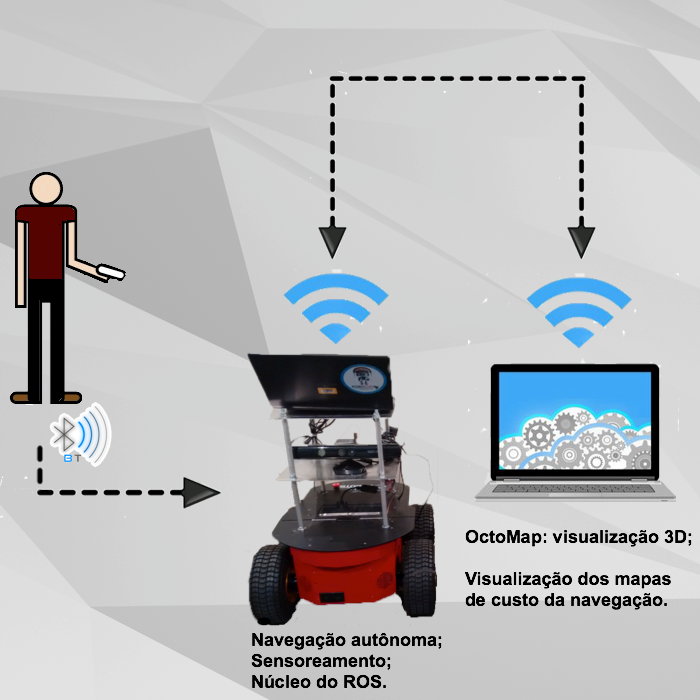
\includegraphics[width=8cm]{images/visaoGeral0.png}
\caption{\small{Visão geral da comunicação no sistema.}}
\label{fig:visaoGeral0}
\end{figure} 

\begin{figure}[H]
\centering
  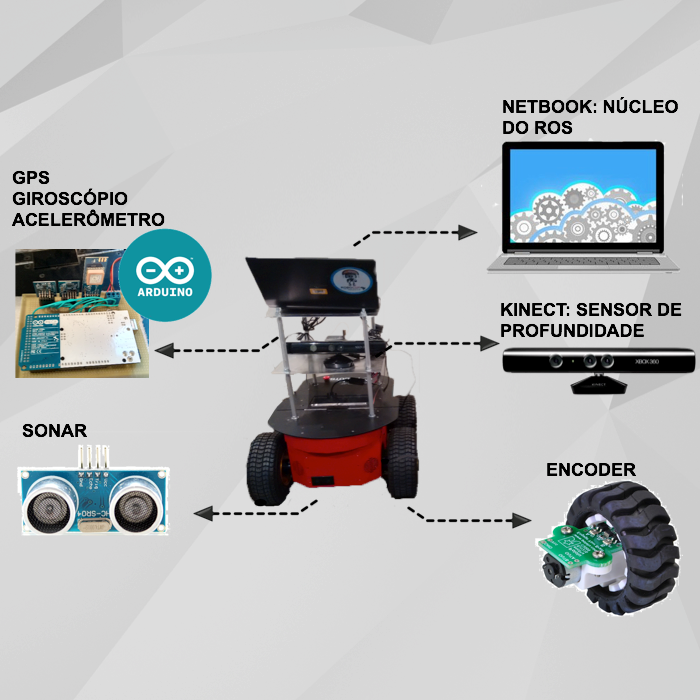
\includegraphics[width=8cm]{images/visaoGeral1.png}
\caption{\small{Visão geral dos sensores do sistema, além do \textit{netbook}.}}
\label{fig:visaoGeral1}
\end{figure} 


Os requisitos funcionais do atual projeto são:
\begin{compactenum}
  \item O robô deve ser teleoperado com um Wiimote, sendo feito o controle de velocidade e direção do robô.
  \item O sistema deve controlar os ângulos vertical e horizontal do Kinect (pan e tilt).
  \item O robô deve navegar autonomamente de forma competente. Considera-se competente uma navegação na qual é possível a detecção de obstáculos baixos e altos, tem-se precisão suficiente para não colidir e é possível um funcionamento prolongado sem necessidade de \textit{reset}.
  \item O sistema deve publicar valores válidos dos sensores (GPS, Acelerômetro e Giroscópio) no ROS.
  \item O sistema deve prover uma visualização tridimensional do ambiente ao redor do robô, enquanto se teleopera o mesmo.
  \end{compactenum}


Os requisitos não funcionais são:
\begin{compactenum}
  \item Uso do \textit{framework} ROS.
  \item Uso do pacote \textit{Navigation Stack} (\verb|move_base| e \verb|gmapping|) para realização do SLAM (\textit{Simultaneous Localization and Mapping}).
  \item Uso do pacote \verb|octomap| para visualização 3D.
  \item Uso das bibliotecas \verb|TinyGPS| e \verb|rosserial| para leitura dos sensor GPS e comunicação entre o microcontrolador e o \textit{master} do ROS.
  \item Uso do microcontrolador Arduino para o controle do servo que gira a base do Kinect, para a leitura dos sensores e para a comunicação com o \textit{master} do ROS.
  \item Uso da biblioteca \verb|wiimote| para comunicação \textit{bluetooth} entre o Wiimote e o ROS.
\end{compactenum}


\section{Desenvolvimento}
\label{sec:desenv}

	\subsection{Teleoperação com o Wiimote}
	\label{sec:desenv:wiiMote}
	
		A teleoperação do robô móvel Pioneer 3-AT foi a primeira parte do projeto desenvolvido. Essa etapa compreendeu o desenvolvimento de três subsistemas:

\begin{compactitem}
\item A comunicação do controle remoto Nintendo Wiimote com o computador mestre do ROS, \textit{framework} de robótica responsável pela integração de todo o sistema.
\item A escrita de um nó, denominação dos processos que rodam usando de funcionalidades do \textit{framework} ROS, para interpretar os comandos vindos do Wiimote e transformá-los em mensagens inteligíveis aos processos que controlam os atuadores do robô, transformando os comandos em ações no mundo real.
\item A escrita de um \textit{launcher} do ROS, arquivo XML que engloba todos os nós usados em um determinado sistema para atingir seus objetivos.
\end{compactitem}

A comunicação do Wiimote com o computador mestre do ROS foi feita usando do pacote \verb|wiimote| ~\cite{wiimote}. Esse pacote permite que, usando-se de comunicação \textit{bluetooth}, nós (\textit{nodes}) estabeleçam comunicação com o controle Wiimote através de tópicos. O pacote foi instalado no sistema fazendo-se \textit{download} do código a partir do repositório fornecido pelos autores ~\cite{gitwiimote} e compilando o mesmo.

A equipe instalou o pacote e conferiu as estruturas das mensagens geradas pelo mesmo, para que fosse possível utilizar com outros nós. Como a documentação não é muito clara, foram feitos testes para descobrir o mapeamento dos botões do controle. 

Entendido o funcionamento básico do pacote \verb|wiimote|, passou-se a desenvolver um nó (em C++), chamado de \verb|wii_oficinas_node| para gerenciar as mensagens do Wiimote, nó este que recebe as mensagens referentes ao estado atual do Wiimote e toma as ações adequadas de acordo com elas. A Figura~\ref{fig:wiimote_botoes} demonstra como os botões e os eixos do giroscópio integrado no Wiimote foram usados para controlar o robô móvel e o Kinect nele integrado. O fluxograma da Figura ~\ref{fig:wii_oficinas_node_flux} (no apêndice) descreve o funcionamento do nó \verb|wii_oficinas_node| e os fluxogramas da Figura ~\ref{fig:ints_wii} descrevem as rotinas de atendimento de interrupção para o nó.

\begin{figure}[H]
\centering
  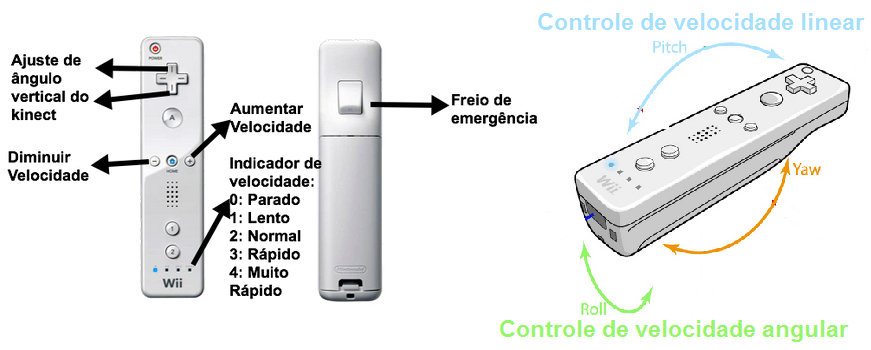
\includegraphics[width=12cm]{images/wiimote_botoes.png} 
\caption{\small{Representação gráfica do uso do controle remoto Nintendo Wiimote para teleoperação do robô móvel Pioneer 3-AT.}}
\label{fig:wiimote_botoes}
\end{figure} 

\begin{figure}[H]
\centering
  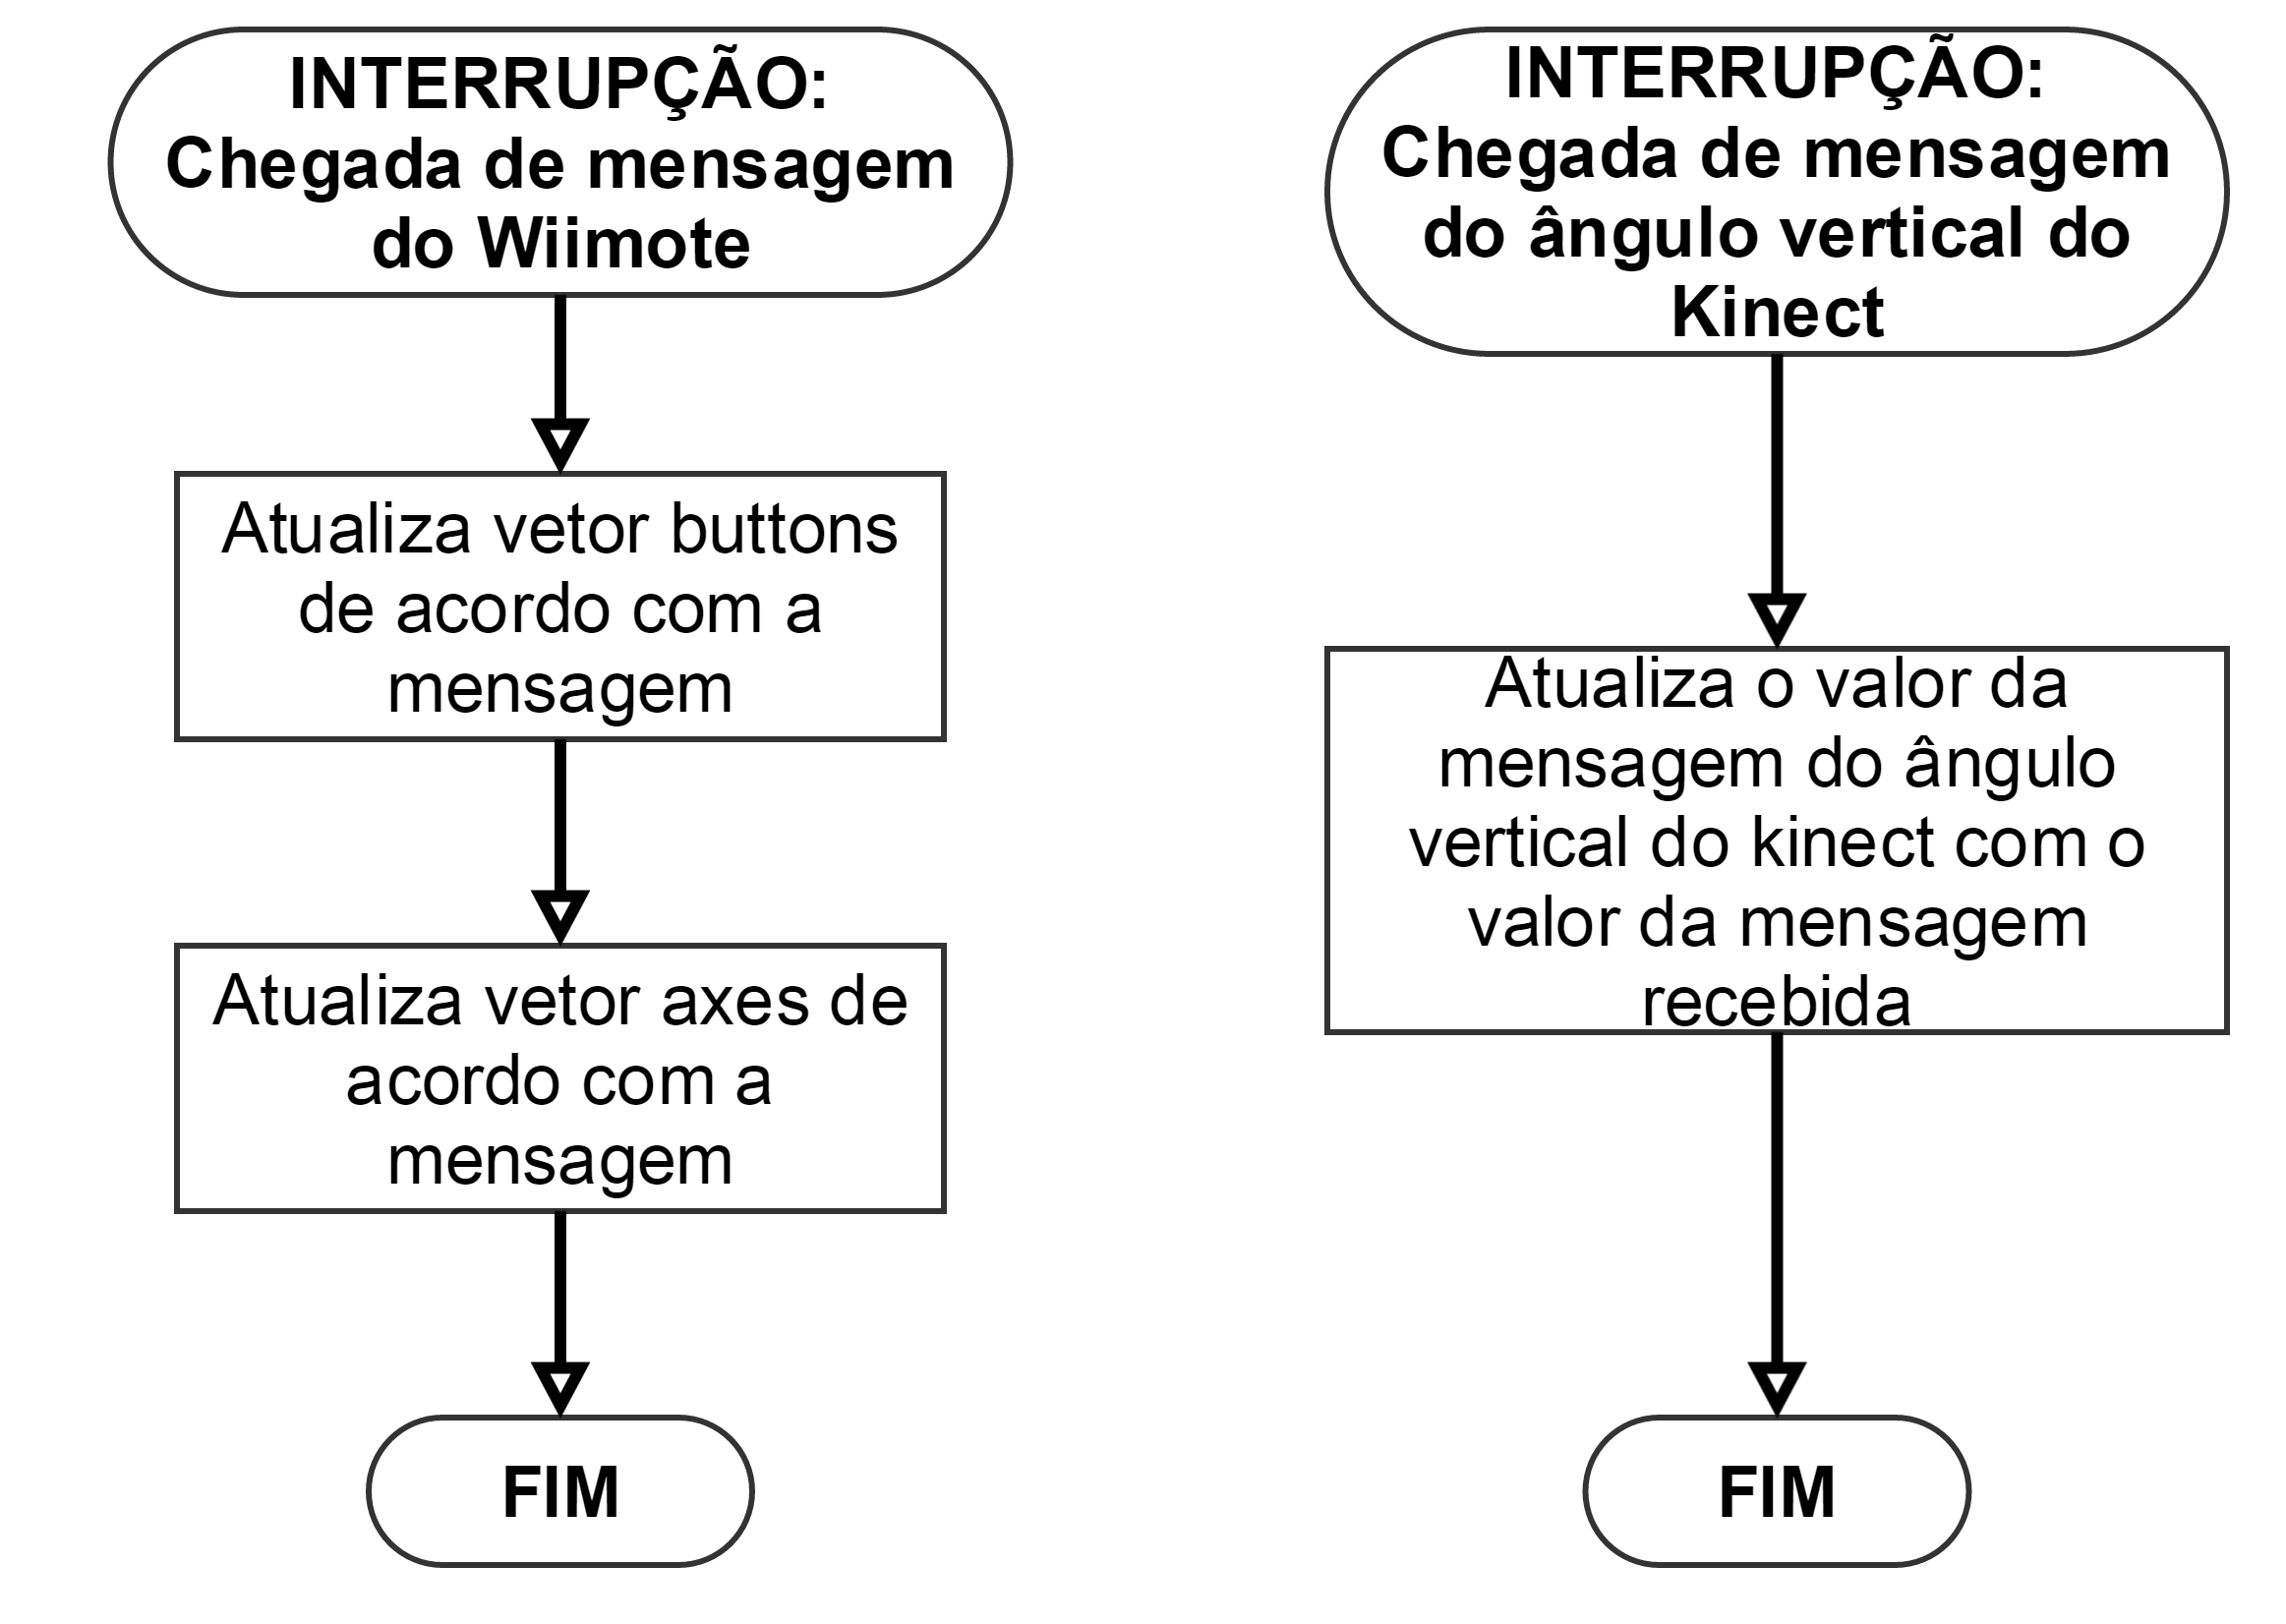
\includegraphics[width=12cm]{images/INTs.png} 
\caption{\small{Fluxograma representando as interrupções geradas pela chegada de mensagens e demonstrando como elas são tratadas.}}
\label{fig:ints_wii}
\end{figure}

		
	\subsection{Interface com Arduino}
	\label{sec:desenv:arduino}
	
		%  /  significa lugares onde tem coisa para dar replace
%  ?? lugares onde estou em duvida.

%Placa
Foi desenvolvida uma nova placa para conexão ao Arduino (\textit{shield}),na qual os seguintes sensores estão dispostos: giroscópio, acelerômetro, GPS e sonar, e ainda um servo motor. A placa foi desenvolvida visando a facilidade e flexibilidade de mudanças no robô, e por isso optou-se por utilizar uma placa perfurada no lugar de um circuito impresso. 

%Sensores
Os sensores utilizados no projeto foram:
\begin{compactitem}
	\item ADXL362 Acelerômetro ~\cite{acelerometro}.
	\item L3G4200D Giroscópio ~\cite{giroscopio}.
	\item GTPA010 GPS ~\cite{gps}.
	\item Sensor Ultrassônico HC-SR04 ~\cite{sonar}.
\end{compactitem}

Com o intuito de facilitar uma futura integração dos dados do acelerômetro e do giroscópio com a navegação autônoma foram definidas APIs (\textit{Application Program Interfaces}) para cada sensor, exceto para o GPS, para o qual foi utilizada uma biblioteca já existente de nome \textit{TinyGPS} \cite{tinyGPS}. Todos os dados obtidos através dos sensores são transmitidos para o computador e publicados em tópicos definidos e, portando, disponíveis ao \textit{framework} ROS. O sonar auxilia na navegação e detalhes da sua utilização e resultados encontram-se na seção ~\ref{sec:result:slam}.

%Motor
O servo motor, modelo MG996R,  é o único atuador presente na placa, e possui a função de rotacionar o Kinect no eixo horizontal. O código implementado se baseia em uma máquina de estados tendo 3 estados possíveis: parado, rotação horária e anti-horária. Estes dados estão disponíveis para o \textit{framework} ROS, assim é possível modificar o estado do algoritmo e acessar a posição atual do Kinect a partir de outro programa que utilize o mesmo \textit{framework}. Para o SLAM e também para o OctoMap (que gera visualização 3D) a posição do Kinect pode ser alterada, mas é preciso informar ao ROS a nova posição do Kinect para que os dados obtidos deste sejam transformados para o novo sistema de coordenadas e continuem coerentes. Foi utilizado o modo \textit{sweep} para o SLAM e também para gerar o ambiente 3D, seus resultados estão nas seções ~\ref{sec:result:octomap} e ~\ref{sec:result:slam}

A API desenvolvida para os sensores consiste basicamente em fazer a leitura dos dados e a escrita deles no respectivo tópico no ROS. Assim, na inicialização dos sensores são configurados os parâmetros desejados e no \textit{loop} principal os dados são lidos e em seguida escritos em seus tópicos.

Já para o motor, a rotina inicial coloca-o na posição 0 (centro) e no estado parado. Em seguida é configurado o temporizador do Arduino para que a cada $25 ms$ o motor atualize sua posição, proporcionando assim um movimento suave. A direção do movimento é determinada pelo programa do Wiimote (sendo executado no ROS). Este programa escreve em um tópico o estado (direção) do movimento e a rotina principal no Arduino lê o mesmo tópico. O fluxograma da Figura \ref{fig:flowchartProgramaArduino} mostra como o programa do Arduino está organizado.

\begin{figure}[H]
\centering
  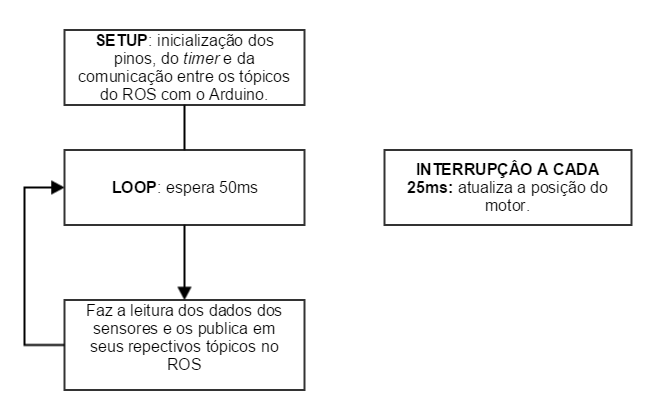
\includegraphics[scale=.5]{images/programaArduino.png} 
\caption{\small{Diagrama de fluxo para o programa executado no Arduino.}}
\label{fig:flowchartProgramaArduino}
\end{figure} 
		
	\subsection{Base para o Kinect}
	\label{sec:desenv:baseKinect}
	
		%  /  significa lugares onde tem coisa para dar replace
%  ?? lugares onde estou em duvida.

Foram resolvidos dois tipos de acoplamento, o do Kinect ao servo motor e o do servo motor ao robô. O objetivo final desta solução era tornar a navegação autônoma mais confiável, pois em certas situações é necessário visualizar as laterais antes de rotacionar o robô. Por isso a necessidade de rotacionar o Kinect, possibilitando "olhar para os lados".

Para solucionar o problema de acoplamento entre o Kinect e o servo motor foram estudadas várias alternativas, entre elas a mais viável foi a encontrada em \cite{modelo3DMotorKinect}. Através do serviço de impressão 3D disponibilizado pelo Departamento Academico de Design Industrial (DADIN) foi possível produzir a peça de acoplamento de forma rápida e barata. O material utilizado na impressão foi o Acrilonitrila Butadieno Estireno (ABS), muito usado para este tipo de serviço. A Figura \ref{fig:modeloMotorKinect} apresenta o modelo no computador e o impresso.

\begin{figure}[H]
\centering
\begin{tabular}{cc}
  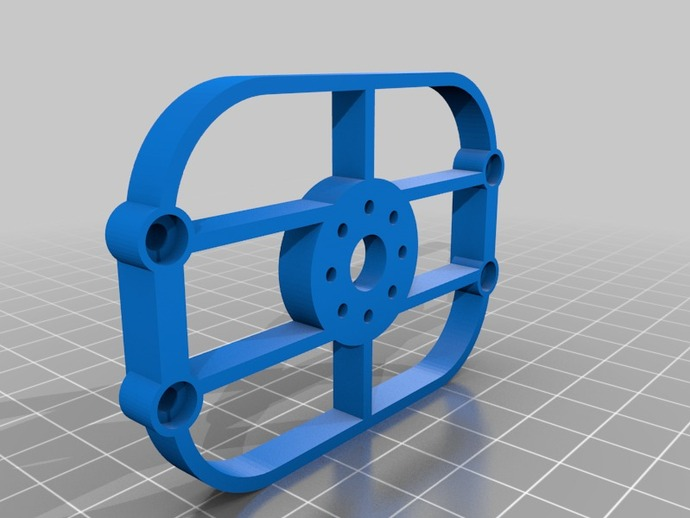
\includegraphics[width=4cm, height=3cm]{images/modeloMotorKinect.jpg} &
  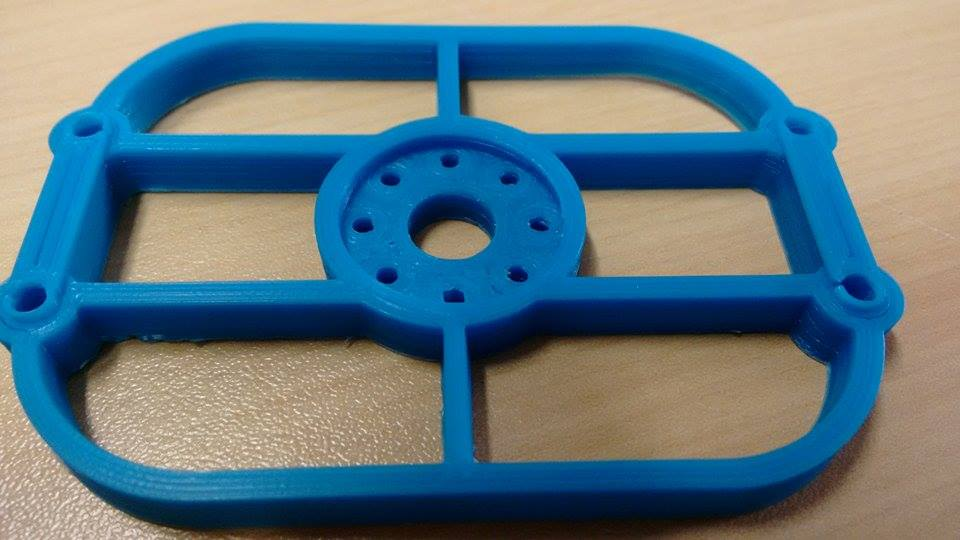
\includegraphics[width=4cm, height=3cm]{images/acoplamentoMotor.jpg} \\
 (a) & (b)
\end{tabular} 
\caption{\small{(a) Modelo sugerido por ~\cite{modelo3DMotorKinect} para acoplar o motor ao Kinect. (b) Peça impressa no DADIN.}}
\label{fig:modeloMotorKinect}
\end{figure} 

O problema de fixação do motor ao robô deveria ser solucionado de forma não invasiva, ou seja, sem alterar a estrutura do robô ou do motor. O projeto para esta peça foi feito no \textit{SketchUp Make 2015}. A Figura \ref{fig:modeloCimaMotorKinect} mostra a peça projetada e a Figura \ref{fig:kinectMontado} apresenta a estrutura final com o Kinect acoplado. Foi escolhida madeira como material para fixar o motor ao robo pois ela é de fácil acesso e manuseio, assim possibilitando o ajuste do modelo durante o projeto.

\begin{figure}[H]
\centering
  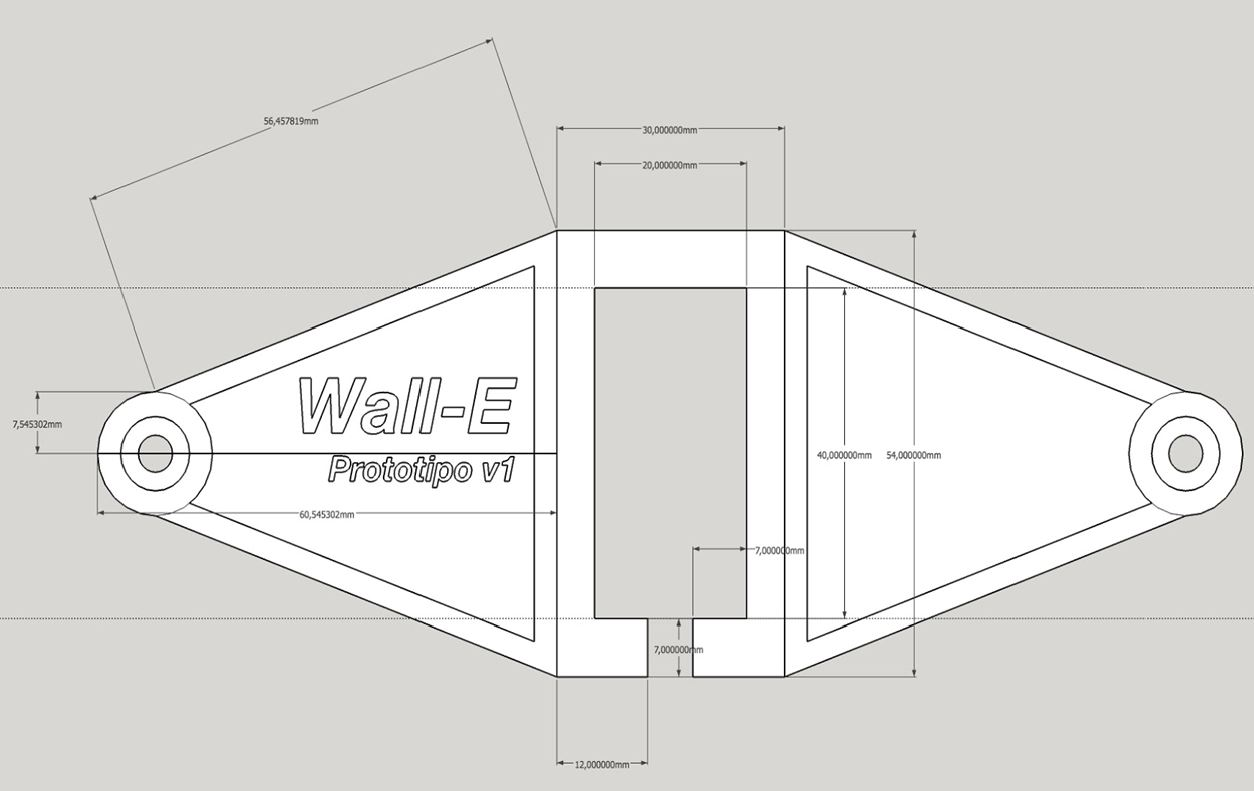
\includegraphics[scale=.35]{images/visaoCimaMotorKinect.jpg} 
\caption{\small{Modelo feito no \textit{SketchUp Make 2015} para acoplar o motor ao robô.}}
\label{fig:modeloCimaMotorKinect}
\end{figure} 


	
	\subsection{Visualização 3D com OctoMap}
	\label{sec:desenv:octomap}
		
		%Muitas aplicações em robótica necessitam de um mapeamento 3D, como visualização de obstáculos e digitalização do estado atual de algum ambiente. 
%PRECISA MESMO DESSA FRASE GENÉRICA AQUI?
O uso do \textit{framework} OctoMap possibilita a geração de modelos tridimensionais de ambientes com a nuvem de pontos gerada pelo Kinect.

Primeiramente foi feito o estudo do código e da documentação do OctoMap. Este \textit{framework} utiliza \textit{octrees}, uma estrutura de dados que permite um melhor uso de recursos como tempo de acesso a memória e tamanho ocupado. Uma \textit{octree} é uma estrutura de dados organizada de forma hierárquica para divisão espacial em 3 dimensões \cite{Wilhelms:1992:Octotrees}\cite{Meagher:1981:Octotrees}. Em uma \textit{octree}, cada espaço é recursivamente dividido em 8 subespaços de mesmo tamanho, até que a densidade de informações por espaço seja a desejada ou se alcance o tamanho mínimo para um espaço. No contexto do OctoMap, cada espaço (também chamado de voxel) apresenta três estados: ocupado, livre e desconhecido.

Para determinar o estado de cada voxel é utilizado a nuvem de pontos gerada pelo Kinect. Voxels ocupados são todos aqueles que possuem pontos em seu interior. Voxels livres são aqueles que não possuem pontos em seu interior e estão entre um voxel ocupado e o sensor. Estes voxels são determinados utilizando um algoritmo de \textit{raycasting} \cite{hornung13auro}. 

O \textit{raycasting} basicamente consiste em traçar um segmento de reta entre o sensor e o voxel ocupado, percorrendo todos os espaços que a reta intersecciona. É neste algoritmo que a estrutura de dados empregada pelo \textit{framework} possui maior importância. Caso os espaços não tivessem nenhuma relação entre si, todos estes deveriam ser testados para determinar se uma interseção ocorreu ou não e esta operação teria um custo de \textbf{O(n)}. No entanto, uma \textit{octree} possui organização hieráquica e apenas um subconjunto dos espaços são testados, resultando em um custo de \textbf{O(log n) }\cite{Havran2000:PhD}.

Entendido o princípio de funcionamento, instalamos o pacote do OctoMap e os \textit{plugins} do \verb|rviz| (sistema de visualização do ROS) para que pudéssemos conferir os resultados. O pacote acompanha um lançador (\textit{launcher}) de demonstração, então antes mesmo de testá-lo, foi criado um lançador em XML que inicializa todas as funções necessárias para seu funcionamento. Esse \textit{launcher} é responsável inicialmente por:

\begin{compactitem}
\item Ligar os \textit{drivers} do Kinect e estabelecer sua comunicação com o ROS.
\item Criar a transformação espacial do sensor Kinect em relação ao centro do robô, referência necessária para o octomap conseguir criar a visualização 3D a partir dos dados.
\item Inicializar o lançador de demonstração do OctoMap.
\end{compactitem}  

Além de criar esse lançador básico, é necessário modificar parâmetros do lançador do OctoMap. São eles:

\begin{compactitem}
\item \textit{Frame} (sistema de coordenadas) de referência fixo, em relação ao qual o OctoMap irá montar os dados. Como não usávamos um sistema de localização no mapa, foi utilizada como referência a odometria do robô.
\item Tópico pelo qual a nuvem de pontos pode ser obtida.
\end{compactitem} 

Em seguida fizemos o lançamento do nosso XML e obtivemos resultados positivos. Fazendo a visualização no \verb|rviz|, o resultado do OctoMap estava dentro do esperado. Em seguida, para a integração do OctoMap com a movimentação do robô e para fazer os dados da visualização acompanhá-los, foram necessárias outras alterações no \textit{launcher}:

\begin{compactitem}
\item Inserção dos nós de comunicação com a base móvel, responsáveis por ligar o robô e interpretar comandos de velocidade.
\item Inserção do nó de comunicação com o Wiimote.
\item Inserção do nó \verb|wii_oficinas_node|, desenvolvido pela equipe para o controle do Kinect e do robô a partir dos comandos do Wiimote.
\item Inserção do nó de comunicação do Arduino com o \textit{netbook}, para receber comandos de movimentação horizontal do Kinect.
\item Inserção do nó \verb|kinect_aux|, responsável pela movimentação vertical do Kinect. 
\end{compactitem} 

Essas modificações foram suficientes para um mapeamento razoável e eficiente do ambiente enquanto o robô era teleoperado com o Wiimote. Os resultados são apresentados e discutidos na seção \ref{sec:result:octomap} (página \pageref{sec:result:octomap}).

%IMPORTANTE: NÃO CITEI NADA DE QUE O OCTOMAP NÃO FUNCIONA SE MEXER O KINECT, MAS SABEMOS QUE, NO ESTADO ATUAL, NÃO FUNCIONA!
	
	\subsection{Navegação autônoma}
	\label{sec:desenv:slam}
	
		No início do projeto, já existia um desenvolvimento em andamento em relação ao SLAM. Entretanto este enfrentava sérios problemas. Os maiores deles eram relativos à localização do rôbo no ambiente e limitações no sensor (Kinect) que não detecta obstáculos próximos (só os detecta em torno de 80 cm). Sendo assim, nossa primeira abordagem buscou resolver o problema de detecção de obstáculos próximos. Não só isso, mas a utilização do \textit{Nuvem de Pontos} do Kinect era limitada por um dos pacotes utilizados, o \verb|gmapping|, que só trabalha com vetores de distância \cite{G_mapping}. Esta conversão causava uma série de perdas de informação, de maneira que a representação virtual do ambiente não condizia com a realidade. 

A proposta inicial foi a adição de um sonar, buscando melhorar a representação virtual do ambiente e tornar menos relevante a limitação do Kinect. Acreditamos, inicialmente, que deveríamos simplesmente adicionar esta fonte de dados ao \verb|gmapping|, configurando este para ter duas fontes de dados, só que descobrimos que isso não é possível, já que o pacote gmapping aceita somente uma. Sendo assim, surgiu a necessidade de fundir os dados do Kinect com os dados do sonar, de maneira que as informações fornecidas ao pacote fossem provenientes só de uma fonte. Inicialmente, queríamos escrever um nó do ROS para fazer esta fusão de dados, mas isto tornou-se muito complexo. Então, buscamos um pacote que ajudasse a fazer esta fusão, encontrando o pacote \verb|ira_laser_tools| que permitiu a fusão e possibilitou a virtualização de scanners a laser. A virtualização faz com que o ROS enxergue várias fontes de dados a partir de uma, no nosso caso uma \textit{Nuvem de Pontos}, sendo estas fontes posicionadas em relação a fonte original, possibilitando a fusão de vários vetores de distância em um só, mais representativo do ambiente. Mais informações podem ser encontradas em \cite{iraLaserTools}.

Utilizando-se deste pacote, a representação do ambiente tornou-se muito mais fiel, detectando uma maior variedade de obstáculos, de maneira que os dados do gmapping se aproximaram da \textit{Nuvem de Pontos}. Essa coerência entre os dados melhorou o funcionamento do sistema de localização.

Nesta etapa, o robô começou a detectar obstáculos onde não existiam. Um dos problemas foi como a equipe configurou a virtualização, em forma de estrela. Este tipo de configuração trouxe erros na navegação, por conta da detecção do chão como obstáculo. Para resolver tal problema, mudamos a configuração para uma série de linhas horizontais, considerando o ponto do Kinect como altura zero. Como estas linhas estão sempre posicionadas na mesma altura, o problema anterior foi eliminado. 

Entretanto, o consumo de CPU do \verb|ira_laser_tools|, é muito alto para o notebook utilizado, o que acabava tornando o processamento de dados muito lento e resultando em perda de informações do ambiente além de eventuais travas totais no sistema. Tivemos que retornar a antiga utilização de uma linha horizontal da \textit{Nuvem de Pontos}, como se fosse um scanner a laser, mas utilizando esta linha para o gmapping \ e o \verb|move_base|, garantindo sincronia entre localização e mapa de custo. Essa modificação melhorou a localização, tornando a detecção de obstáculos confiável e a integração entre o gmapping e o \verb|move_base| se tornou mais efetiva, viabilizando a utilização do gmapping.

Nesta etapa, a base para movimento angular do Kinect estava completa, então decidimos integrar a movimentação do Kinect para tentar obter um maior ângulo de visão. O Arduino já estava controlando a movimentação do servo-motor que rotacionava o Kinect, então criamos um nó do ROS que girava o motor de forma a fazer uma varredura do ambiente. A comunicação do Arduino dá como feedback o ângulo horizontal atual do servo-motor, valor necessário para configuração de uma transformada geométrica dinâmica da posição a partir da qual os dados do Kinect são obtidos. Infelizmente, os erros cumulativos desta abordagem se provaram muito grandes para que ela fosse útil, causando detecção de obstáculos onde os mesmos não existiam e prejudicando a funcionalidade do gmapping, fazendo com que o robô não conseguisse nem detectar objetos nem se localizar no ambiente.

Após algumas tentativas percebemos outro problema, que a equipe considerou mais impactante: o planejador de rotas local não estava seguindo uma rota condizente com a do planejador global. A rota planejada pelo planejador global era adequada, mas o local não a seguia, ignorando-a completamente. Como é o planejador local que controla o robô, a navegação autônoma não funcionava corretamente, colidindo em obstáculos e traçando rotas que não levariam o robô ao destino desejado se fossem completadas. Assim, decidimos fazer uma troca do planejador de rotas locais do padrão \verb|move_base| para o \verb|dwa_local_planner|, mais indicado para nosso robô como visto em \cite{dwaLocalPlanner}. Esta troca trouxe melhorias nas áreas citadas, trazendo rotas condizentes com o planejador global e que levavam ao local desejado. 
%Com as rotas adequadas, percebemos que as rotas traçadas ficavam muito perto era necessário ainda tínhamos problemas, pois o robô passava perto demais dos obstáculos ou batia nos que estavam fora de seu ângulo de visão, problema este que pode ser resolvido pela varredura, numa eventual continuidade do projeto.  

Nesta etapa, a equipe modificou alguns parâmetros com relação ao mapa de custo gerado. O mapa de custo é parte da navegação autônoma, sendo construído pelos sensores de maneira dinâmica neste caso. Ele é uma representação bidimensional do ambiente, sendo gerada uma matriz com valores de 0 a 255. Quando um sensor detecta um obstáculo, aquele ponto no mapa 2D é marcado com o valor 255 e custos em torno deste ponto são marcados com valores menores, decaindo de acordo com uma exponencial, até chegar ao raio determinado, onde o custo será 0. O parâmetro do raio é chamado \verb|inflation_radius| e a exponencial de decaimento é determinada utilizando o \verb|cost_scaling_factor|.  Mais informações podem ser encontradas em \cite{costmap2D}.

No pacote de visualização do ROS, o \verb|rviz|, podíamos ver que a rota traçada era agora condizente com os custos do mapa, mas que a área de alto custo em volta dos obstáculos era pequena em relação ao robô, o que fazia com que este passasse muito perto ou até colidisse com os obstáculos. Quando mudávamos o parâmetro \verb|inflation_radius|, que dá o raio de alto custo em volta dos obstáculos, não conseguíamos aumentar o tamanho dessa área. Descobrimos que para o funcionamento correto, deveríamos ter uma combinação adequada de \verb|inflation_radius| e \verb|cost_scaling_factor|. Feitas essas modificações, conduzimos novos testes, nos quais se verificou uma melhora significativa. Nessa fase, o robô é capaz de desviar os obstáculos presentes no mapa de custo global, traçar rotas globais e locais condizentes com os mapas de custo e atingir a maioria dos \textit{goals} com certa uma margem de erro aceitável. Infelizmente, durante esse processo, existe um certo erro no encaixe entre os mapas de custo local e global, que é corrigido pelo sistema de localização \verb|gmapping| em tempo, na maioria das vezes, aceitável. 

Fazendo uma revisão de todos os parâmetros da navegação, chegamos em alguns parâmetros que poderiam nos ajudar a fazer uma melhor localização usando do pacote gmapping. Esses parâmetros eram:

\begin{compactitem}
\item \verb|iterations|: Esse parâmetro seleciona o número de iterações que o gmapping fará para tentar encaixar os dois mapas. Antigamente era feita apenas uma iteração, agora são 5.
\item \verb|srr,str,stt e srt|: Esses quatro parâmetros dizem respeito a confiabilidade da odometria. Quando o gmapping vai fazer a transformação que corrige os erros da odometria, é essencial que ele saiba os erros máximos esperados, de forma a não chutar erros altos demais. Medimos esses erros em uma etapa anterior ao trabalho de oficinas 3, mas projetos com robôs parecidos indicavam valores muito menores aos que usávamos. Diminuímos todos esses parâmetros em cerca de dez vezes.
\item \verb|particles|: O gmapping é um sistema de localização baseado no método de monte carlo, e para achar a posição do robô no ambiente posiciona aleatóriamente várias partículas no ambiente, vendo qual delas é a mais próxima da posição real do robô. Mudamos esse parâmetro de 30 para 300, aumentando muito a precisão do pacote.
\end{compactitem}

A mudança desses três parâmetros deixou o robô com uma navegação muito perto da que esperávamos, sendo que o robô chegava em praticamente todos os destinos para o qual mandávamos. Percebemos que o único caso que ele não conseguia chegar ao destino era quando precisava dar ré, todos os outros casos de teste funcionaram. Procuramos mais um pouco dentre os parâmetros e vimos que o padrão para o \verb|dwa_local_planner| era que a velocidade linear mínima fosse de 0, ou seja, não deixava o robô andar de ré. Mudamos esse parâmetro e, após as modificações, obtivemos os resultados esperados: o robô conseguiu se movimentar com razoável precisão em todos os cenários que o testamos, com repetibilidade e sem cometer grandes erros.

\section{Resultados e discussões}
\label{sec:result}

	\subsection{Teleoperação com o Wiimote}
	\label{sec:result:wiiMote}
	
		Foram verificadas todas as principais funcionalidades deste sistema e, assim, feitos ajustes empíricos que resultaram em um melhor desempenho no controle do robô e do Kinect conforme descrito abaixo:

\begin{compactitem}
\item Quando o controle e o computador se conectam (pareiam), ele vibra. Empiricamente, ajustamos a vibração para uma duração que possa ser percebida, mas que não seja desconfortável.
\item Assim que o controle liga, nenhum LED está aceso, e ele se encontra na velocidade 0. Nesse estado, não é possível mover o robô, independente de como o Wiimote é movimentado.
\item Os botões \verb|+| e \verb|-| do Wiimote são responsáveis por trocar entre as velocidades 0 e 4. Esta funcionalidade foi extensivamente testada e em nenhum caso \textit{bugs} foram detectados, sendo que todos os LEDs acendiam corretamente e percebia-se a mudança de velocidade entre os estágios.
\item Nos estados de velocidade 1 a 4, o robô se move proporcionalmente à inclinação do Wiimote. Ajustamos os fatores multiplicativos de cada nível de velocidade de forma a buscar uma curva de aceleração que permita um bom controle do robô em todos os estágios, além de haver uma clara mudança de velocidade entre os estágios.
\item O botão \verb|B| é responsável por frear o robô instantaneamente e colocá-lo no estado de velocidade 0, independente de sua configuração atual do robô. Testamos essa funcionalidade nos mais diversos cenários e não encontramos nenhum problema.
\item As setas direcionais para cima e para baixo são responsáveis por regular o ângulo vertical do Kinect. Em princípio, esse controle era bem difícil de ser obtido e o Kinect continuava se movendo por bastante tempo após o botão ter sido liberado. Fizemos alguns ajustes no código e testamos abordagens diferentes para a publicação do ângulo do Kinect para o pacote \verb|kinect_aux|, chegando no atual, que se mostrou a melhor forma de controle.
\item As setas direcionais para esquerda e direita são responsáveis por regular o ângulo horizontal do Kinect. Esse controle também não atuou como esperávamos, principalmente em função da demora da transmissão dos dados do Wiimote para o Arduino e pela imprecisão no posicionamento do servo. Não era possível mover o motor de maneira contínua, sendo que este apresentava saltos discretos entre posições vizinhas, as duas abordagens que apresentaram melhores resultados foram:
\begin{compactitem}
\item Quando um botão direcional for pressionado, enviar para o Arduino um comando com o lado para o qual deve girar e, quando o botão for solto, mandar um comando de parada. Dessa forma, o atraso não é tão perceptível e o Arduino consegue lidar com passos discretos bastante pequenos (suficientes para não serem notados).
\item Dividir o percurso total do servo motor em poucos passos discretos, que podem ser escolhidos com cliques nos direcionais, ou seja, um toque para a esquerda resulta em um único movimento de X graus. Nossa preferência foi usar X igual a 10 graus, fazendo com que o servo-motor tivesse 13 passos em seus 120º totais de percurso.
\end{compactitem} 
\end{compactitem}

A versão atual do \textit{software} do Wiimote apresenta todas as funcionalidades propostas: movimentar o Kinect nos eixos vertical e horizontal, movimentar o robô e adicionalmente incluimos duas funções: \textit{sweep}, que percorre continuamente os 120 graus possíveis do servo motor e \textit{home} que movimenta o Kinect para o centro (Kinect direcionado para frente).
		
	\subsection{Sensores}
	\label{sec:result:sensores}
	
		Os dados obtidos dos sensores em testes de posicionamento e movimentação foram condizentes com a realidade, no entanto não foram realizados testes para determinar a precisão dos sensores. Todos os dados são publicados em tópicos do \textit{framework} ROS e estão disponíveis para qualquer programa que o utilize.

O acelerômetro e o giroscópio são publicados no tópico do tipo TWIST (tipo de mensagem usada pelo ROS). Este tipo de mensagem é específico para a transmissão de informações a respeito da velocidade linear e angular de um objeto. Seus dados podem ser facilmente verificados fazendo uso de uma ferramenta do ROS, chamada de \textit{rostopic}, sendo necessário apenas solicitar o comando: \verb|\$ rostopic echo /nome_do_topico|.

O sonar é publicado em um tópico do tipo \textit{float}. Seus dados foram inicialmente usados para mitigar a limitação de alcance do Kinect, que só consegue perceber objetos a partir de aproximadamente $80cm$. Entretanto, o custo computacional de mesclar os dados do sonar com os do Kinect foram superiores ao esperado, tornando sua utilização pouco efetiva no SLAM.	
	
	\subsection{Movimentação do Kinect}
	\label{sec:result:movKinect}
	
		As soluções empregadas na fixação do motor ao robô e do Kinect ao motor foram satisfatórias pois a movimentação ficou suficientemente suave para sua possível utilização tanto na navegação autônoma quanto no mapeamento 3D. Por mais que o servo motor apresente erros ao manter sua posição este não foi suficiente para prejudicar as leituras do Kinect.

A utilização de interrupções no tempo para movimentar o motor foram essenciais para que o mesmo fizesse movimentos mais suaves, aperfeiçoando o controle de posição com o Wiimote. A Figura \ref{fig:kinectMontado} mostra o Kinect já acoplado ao motor e o motor ao robô.

\begin{figure}[H]
\centering
  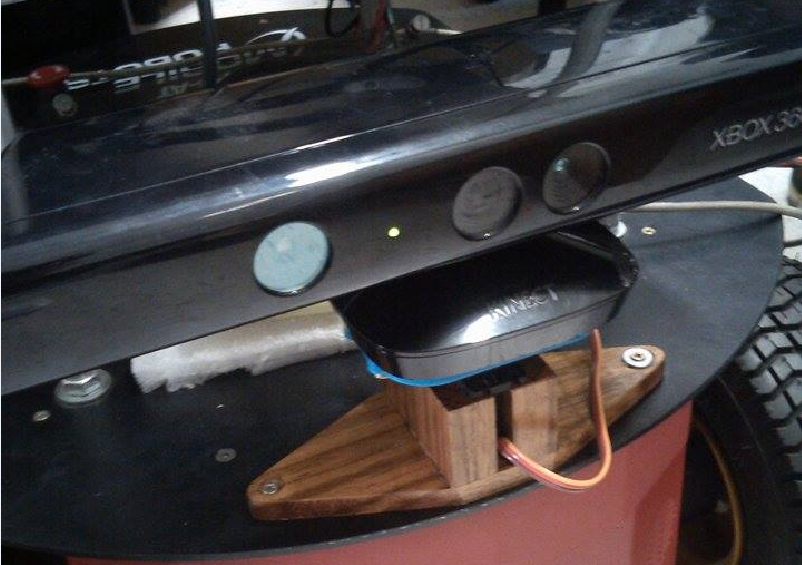
\includegraphics[scale=.35]{images/kinectMontado.png} \\
\caption{\small{Estrutura final de fixação do Kinect.}}
\label{fig:kinectMontado}
\end{figure} 	
	
	\subsection{Visualização 3D com OctoMap}
	\label{sec:result:octomap}
		
		A Figura ~\ref{fig:cadeiraOctomap} apresenta um exemplo dos resultados obtidos com o uso do pacote \verb|octomap|. Em ~\ref{fig:cadeiraOctomap}(b) é mostrada a cena capturada pela câmera convencional do Kinect e, em ~\ref{fig:cadeiraOctomap}(a) a saída do OctoMap. É possível verificar a precisão deste método sabendo que cada quadrado tem resolução de $5cm$, escolhido no \textit{launcher} do OctoMap, e a cadeira tem $40cm$ de largura. Após a contagem dos quadrados, podemos concluir que o modelo gerado está muito próximo do real pois o encosto tem 9 quadrados de largura.

\begin{figure}[H]
\centering
\begin{tabular}{cc}
  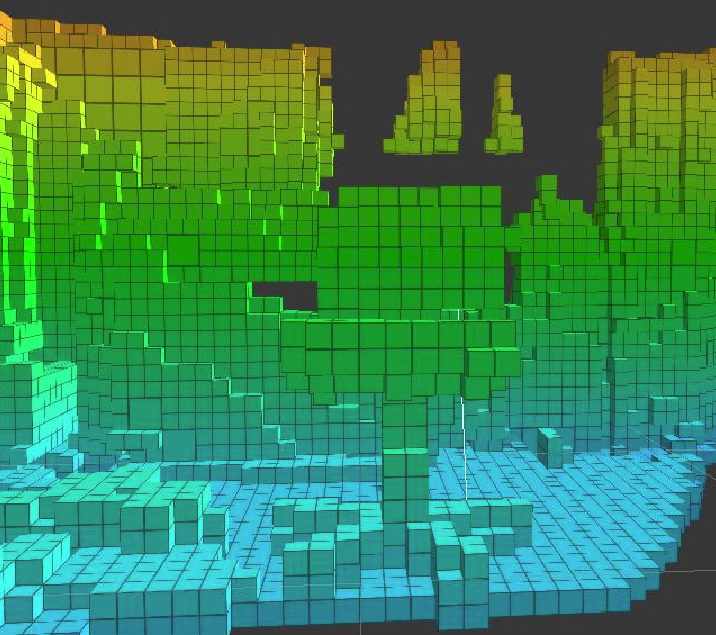
\includegraphics[width=6cm, height=6cm]{images/cadeiraOctomap.PNG} &
  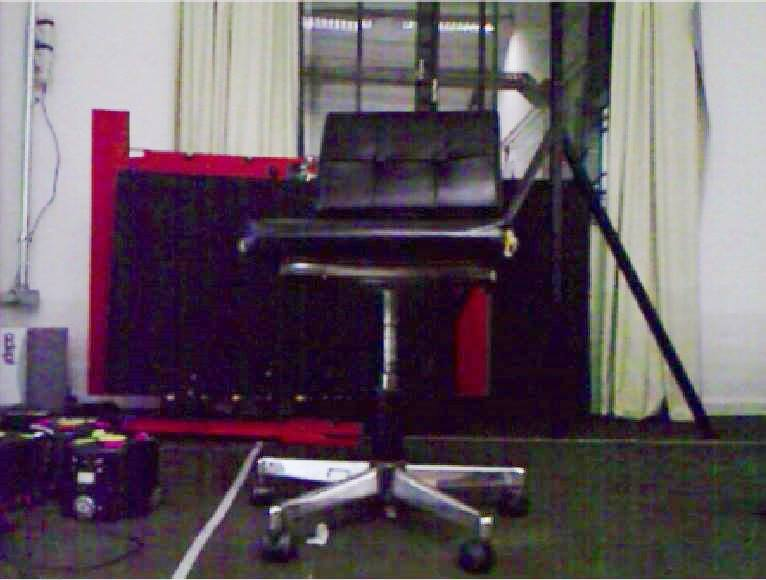
\includegraphics[width=6cm, height=6cm]{images/cadeiraKinect.jpg} \\
 (a) & (b)
\end{tabular} 
\caption{\small{(a) Resultado obtido com OctoMap \cite{hornung13auro}. (b) Imagem capturada da câmera do Kinect.}}
\label{fig:cadeiraOctomap}
\end{figure}

Foram feitos testes com o pacote e ele se mostrou eficiente computacionalmente, sendo possível mapear ambientes internos de diferentes tamanhos sem grandes problemas, mesmo no \textit{netbook}, que é o \textit{master} do ROS. Quanto aos problemas, foram encontrados alguns erros percetíveis ao fazer o mapeamento dos ambientes de teste:

\begin{compactitem}
\item Muitas vezes, ao fazer o mapeamento de algum local o pacote  marca um mesmo objeto duas vezes em posições ligeiramente diferentes, poluindo a visualização e não representando fielmente a realidade. Esse problema se repete até mesmo em ambientes simulados e trata-se de um problema conhecido do pacote. Neste momento, uma melhoria neste comportamento encontra-se fora do escopo do projeto.
\item Nos primeiros testes o sistema de coordenadas de referência considerado era o \verb|odom| (responsável pela odometria), sendo que os erros cumulativos de odometria causavam erros, algumas vezes, consideráveis. Para fim de testes, foi usado o sistema de localização \verb|gmapping| (em parte responsável pelo SLAM) e adotado o sistema de coordenadas de referência \textit{map} (criado pelo \verb|gmapping|), o que não trouxe melhoras significativas.
\end{compactitem}
	
	\subsection{Navegação autônoma}
	\label{sec:result:slam}
	
		Escolhemos como cenário de teste uma sala com alguns obstáculos, conforme mostrado na Figura ~\ref{fig:nav}. Fizemos então um nó (em C++) que publica dois \textit{goals} para o \verb|move_base|, no qual o caminho mais próximo seria colidindo em objetos do ambiente. Conduzimos os testes e chegamos às seguintes conclusões:
\begin{compactitem}
\item Os obstáculos, além de uma área em volta deles, eram corretamente evitados pelo robô, que fazia o máximo para gerar um caminho seguro que chegasse ao seu destino. 
\item O robô atualiza frequentemente seu caminho, buscando melhores alternativas conforme vai melhor reconhecendo o ambiente.
\item Os mapas de custo global e local apresentavam dados condizentes entre si e também condizentes com o que era mostrado no mapa criado pelo \verb|gmapping|. Na Figura \ref{fig:nav}, o que se vê é o mapa local, já que ele está quase perfeitamente encaixado com o mapa global, que está por baixo. Se olharmos no canto superior da imagem, podemos ver uma pequena porção do mapa global, da mesma coloração do local, mas bem mais claro. Não é possível perceber a diferença entre o local e o global na Figura \ref{fig:costmap} e na Figura \ref{fig:nav} já que os dois estão praticamente perfeitamente sobrepostos. Este é o resultado desejado, sendo que erro na sobreposição dos mapas implica em erros na navegação.
\item Devido aos erros da odometria, o mapa de custo local 'desliza' sobre o mapa de custo global. Após algum tempo, o \verb|gmapping| publica uma nova transformação entre os \textit{frames} do mapa e do \verb|odom| e corrigia esse erro, realinhando os mapas.
\item Nos testes, vimos também que o ângulo de visualização bastante fechado do Kinect limita muito o seu funcionamento e faz o robô ter muita incerteza quanto ao ambiente. Esse sensor se mostrou inferior aos sensores scanners a laser de distância para essa aplicação.
\end{compactitem} 

\begin{figure}[H]
\centering
  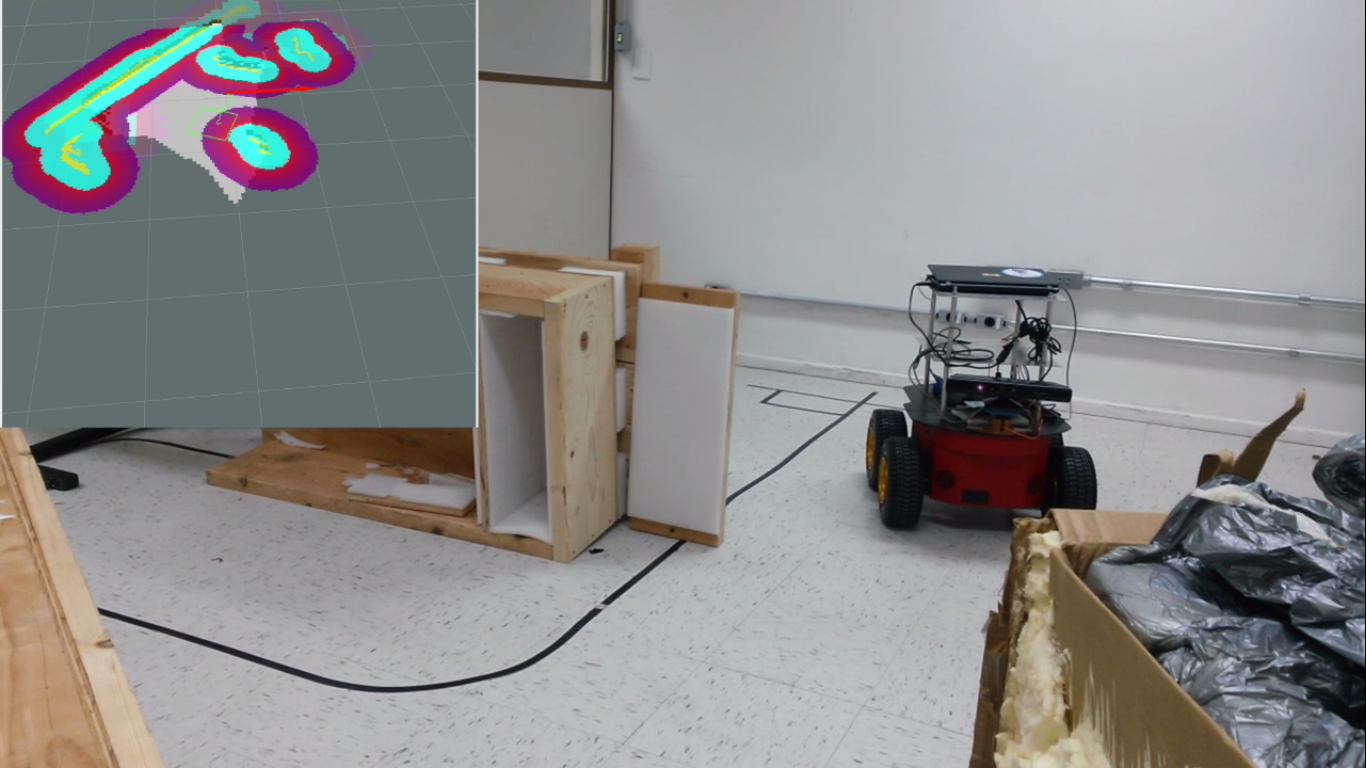
\includegraphics[width=12cm]{images/nav.png} 
\caption{\small{Robô móvel Pioneer 3-AT navegando no cenário de testes. No canto esquerdo superior é possível ver o mapa de custo gerado, além do \textit{footprint} do robô e da trajetória atual.}}
\label{fig:nav}
\end{figure}

\begin{figure}[H]
\centering
  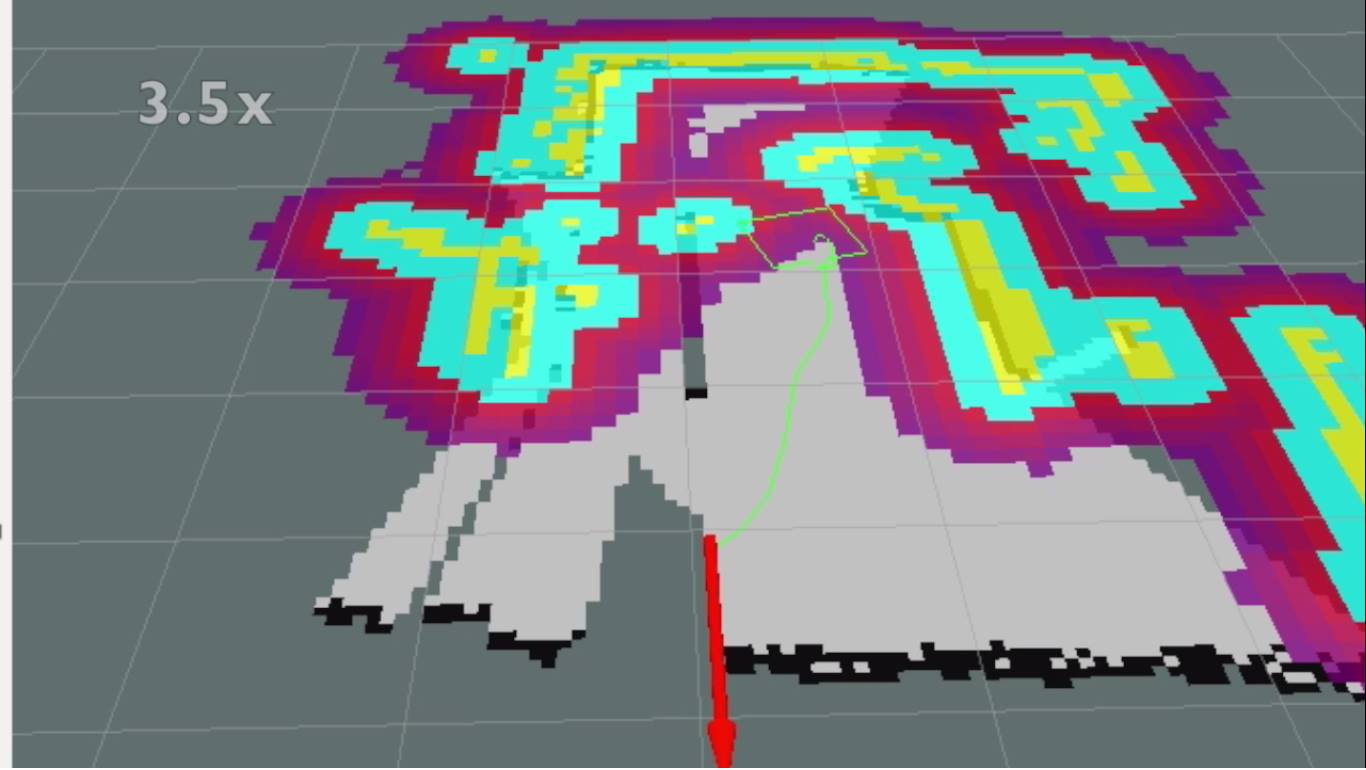
\includegraphics[width=12cm]{images/MapaCusto.png} 
\caption{\small{Imagem detalhada de um exemplo de mapa de custo em um cenário de teste. Os mapas de custo local e global estão perfeitamente sobrepostos na imagem, sendo este um resultado ótimo. A linha preta delimita áreas de mudança de mapa local para mapa global, sendo o global o maior dos dois.}}
\label{fig:costmap}
\end{figure} 
 
\section{Considerações finais}
\label{sec:conc}

A equipe acredita que todos os objetivos da disciplina foram cumpridos, desde a comunicação sem fio, como o trabalho com \textit{hardware} e \textit{software}. Tivemos resultados favoráveis e todas as melhorias realizadas e documentadas irão auxiliar ao longo do desenvolvimento do projeto nos semestres que seguem, considerando que este trabalho foi uma extensão da iniciação científica de um dos integrantes, sentimos que o aspecto de proporcionar vias de melhorias futuras é muito interessante, além da documentação presente aqui para possível compartilhamento com a comunidade.

Um dos focos do grupo foi a abordagem de como as limitações dos sensores utilizados, principalmente do Kinect, podem ser superadas de maneiras menos custosas, buscando sempre uma relação custo-benefício alta. Podemos perceber isso analisando o custo dos equipamentos presentes no ínicio do projeto e o custo de nossas melhorias, disponibilizados na Tabela \ref{tab:custoAnterior} e o custo envolvido no aprimoramento deste sistema está na Tabela \ref{tab:custoNosso}.


\begin{table}[h]
\caption{\small{Custo dos equipamentos já presentes no projeto.}}
\begin{center}
\begin{tabular}{c|c}
\hline
Descrição & Valor em reais \\
\hline
Kinect & 300,00 \\ 
Controle de Wii e adaptador \textit{bluetooth} & 100,00 \\  
Robô Pioneer 3-AT & 18.000,00 \\ 
\textit{Netbook} & 700,00 \\
Arduino Mega 2560 & 90,00 \\
\hline
Total & 19.190,00 \\
\hline
\end{tabular}
\end{center}
\label{tab:custoAnterior}
\end{table}

\begin{table}[h]
\caption{\small{Custo para o aprimoramento.}}
\begin{center}
\begin{tabular}{c|c}
\hline
Descrição & Valor em reais \\
\hline
Materiais para a nova placa do Arduino & 10,00 \\ 
Servo motor MG996R & 55,00 \\  
Estrutura para o Kinect & 15,00 \\ 
\textit{Hub} USB 2.0 & 10,00 \\
\hline
Total & 80,00 \\
\hline
\end{tabular}
\end{center}
\label{tab:custoNosso}
\end{table}

Ao compararmos o custo total de equipamentos que já estavam presentes no projeto ($19.190,00$ reais) e o custo total para o aprimoramento ($80,00$ reais) percebemos como o pequeno investimento monetário tornou possível adicionar as funções de: teleoperação com um Wiimote do robô e da posição da câmera do Kinect, mapeamento 3D, assim como melhorias na navegação autônoma. 

Desta forma, acreditamos que o trabalho realizado apresenta muitas opções para o futuro do projeto como um todo, algo muito vantajoso quando se pensa na natureza de melhoria contínua do mesmo. Acreditamos que com a descoberta de pacotes como o \verb|ira_laser_tools| e a utilização de um computador com melhores configurações é possível gerar resultados ainda melhores.

Outrossim, por mais que ainda existam inconvenientes na navegação autônoma, como falta de repetibilidade, ou até mesmo erros de má localização, houve melhoras signficativas neste projeto (seção \ref{sec:result:slam}). A visualização 3D do ambiente foi possível, mas ainda pode apresentar erro quando um mesmo objeto é mapeado duas vezes em tempos diferentes, pois por conta do erro da odometria a referência para gerar os dados muda.

Buscamos também, que todo o desenvolvimento aqui documentado permita um desenvolvimento aguçado nos próximos semestres, tornando a compreensão de configurações, pacotes, \textit{plugins} e sensores facilitada. As limitações e dificuldades citadas ao longo deste documento buscam motivar melhorias futuras e tornar a navegação autônoma e a visualização 3D ainda mais eficiente. Esperamos que o trabalho contribua para o desenvolvimento de uma excelência em robótica na nossa universidade. Por fim, o cronograma foi cumprido e os objetivos propostos alcalçados, conforme demonstraram os testes de navegação realizados com o robô em um ambiente interno.

%Insere referencias [---
\bibliographystyle{alpha}
\bibliography{IF66J} % Substituir pelo seu arquivo bib

\section*{Apêndice}
	\begin{figure}[h]
	\centering
  		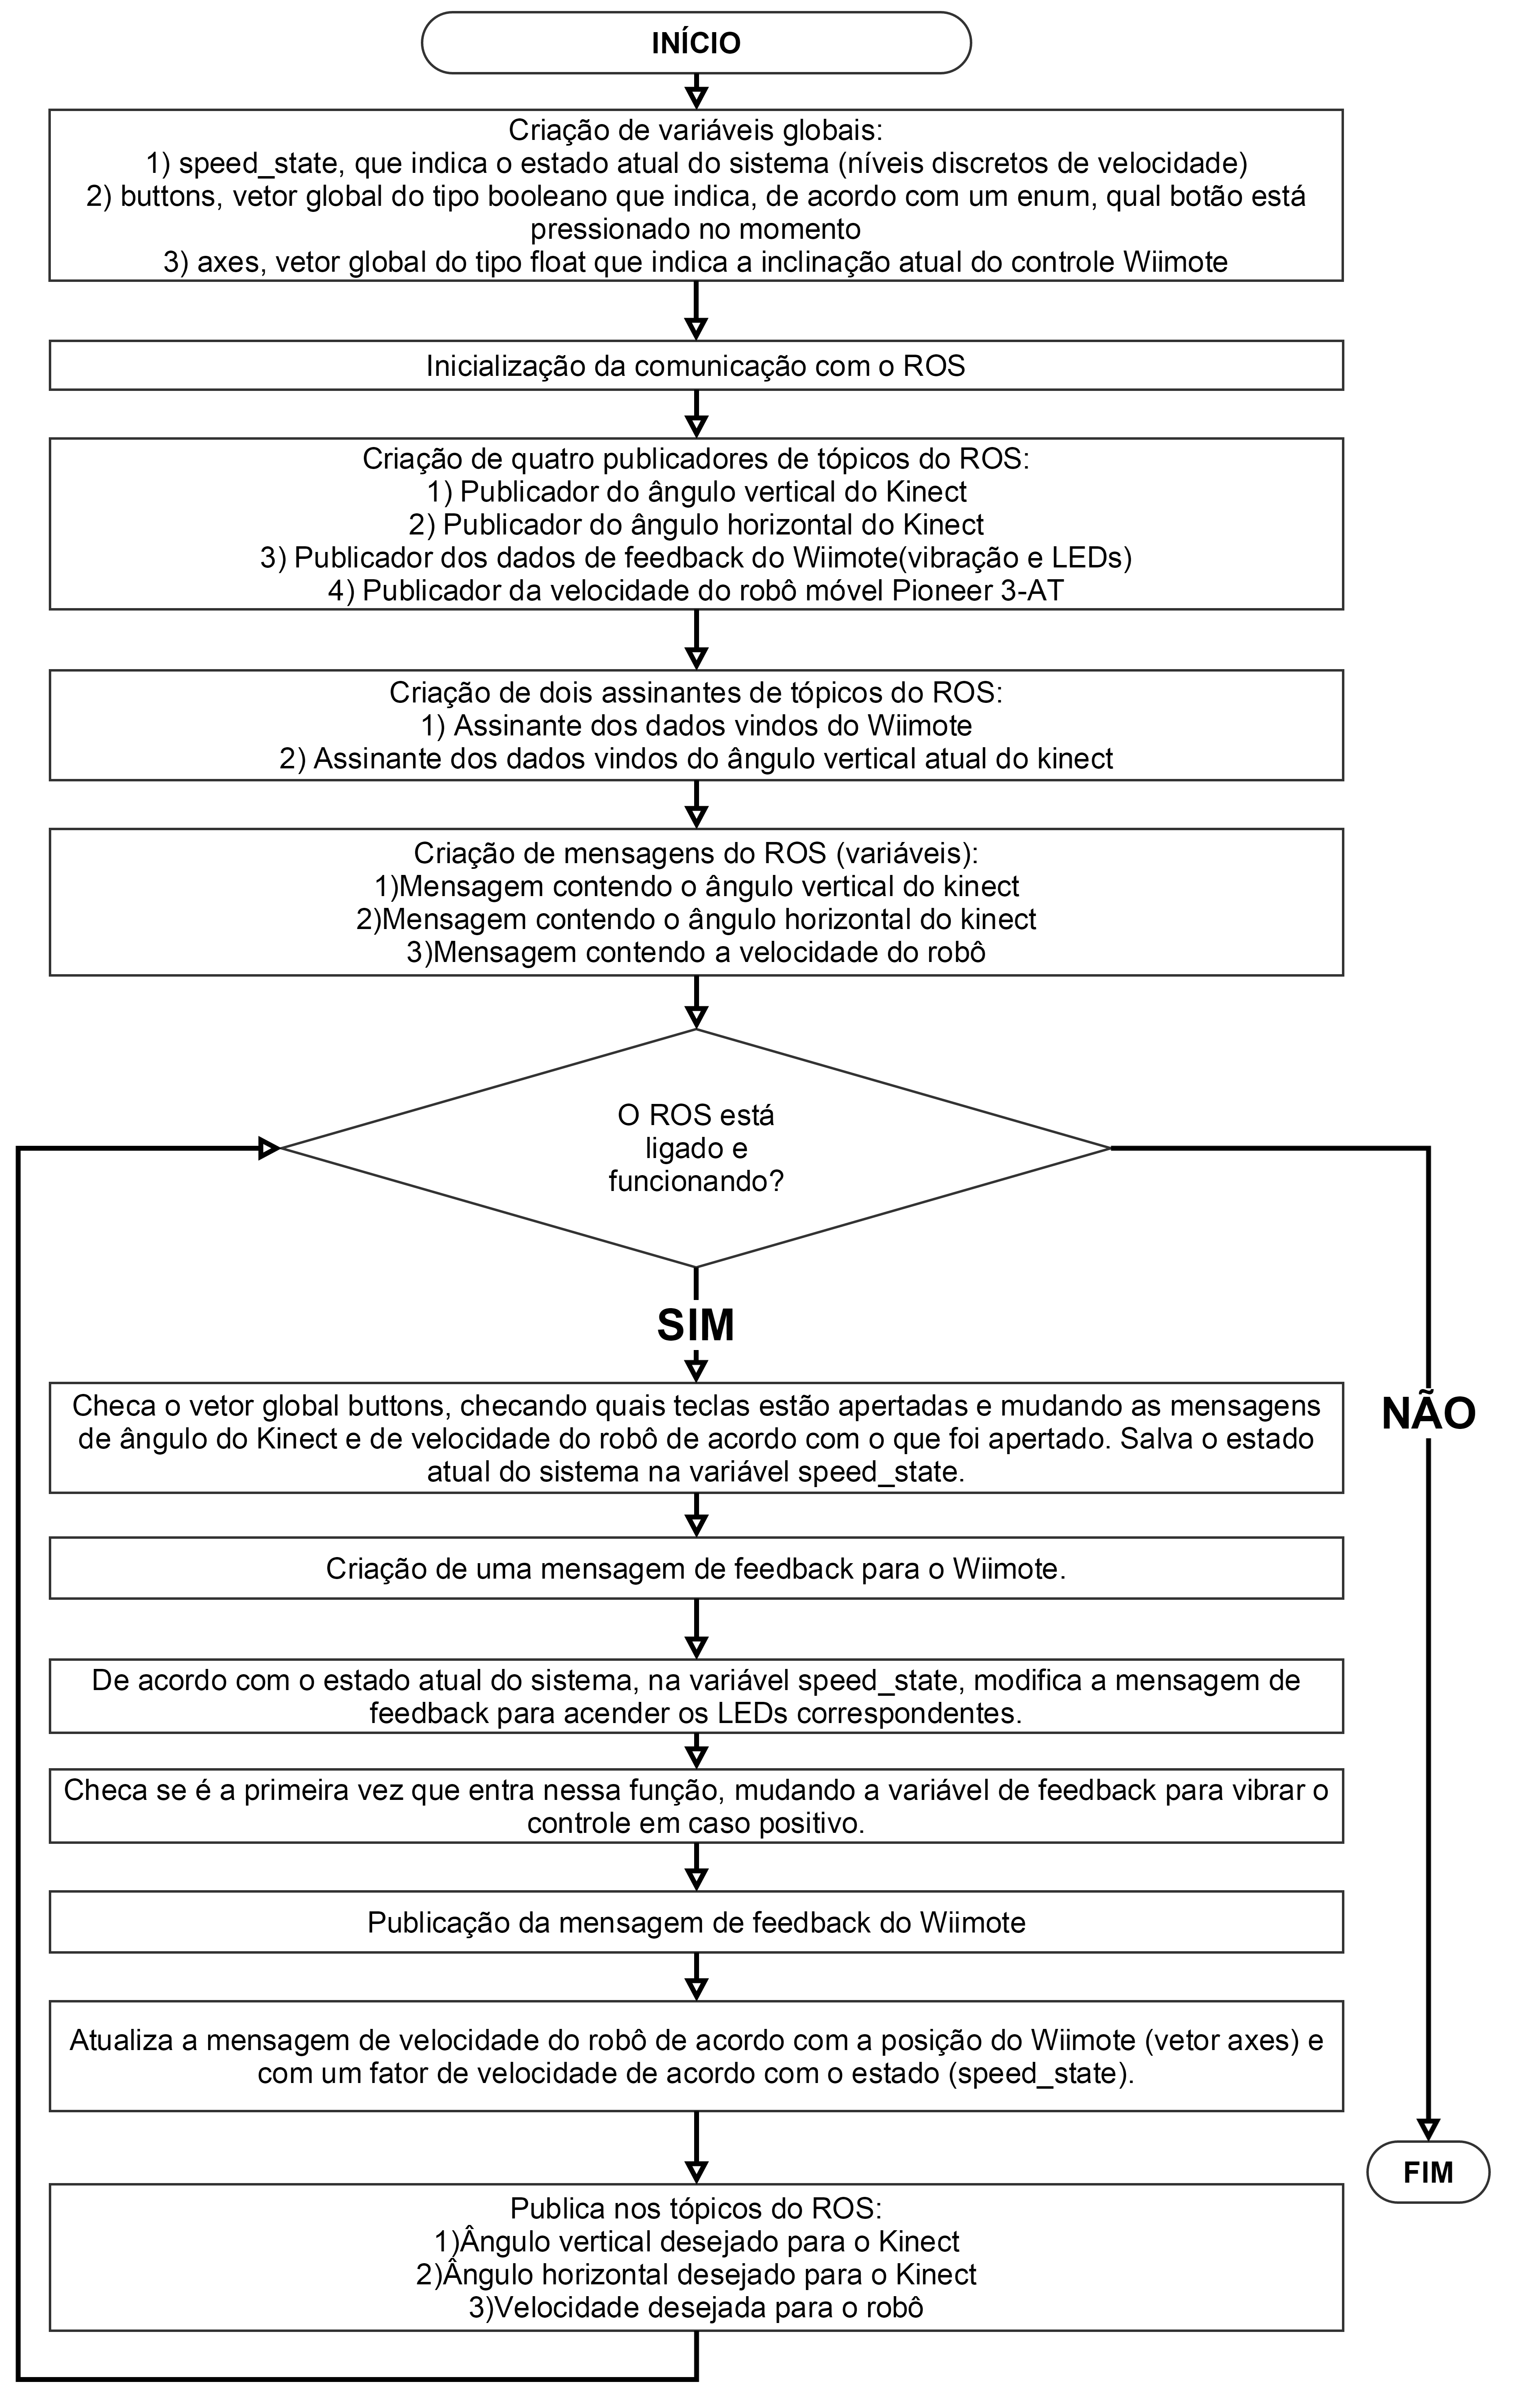
\includegraphics[height=19cm]{images/wii_oficinas_node_flux.png} 
		\caption{\small{Fluxograma representando o funcionamento geral do programa wii$\_$oficinas$\_$node, que se comunica com o controle Wiimote e controla o robô móvel de acordo com as mensagens que recebe. Note que as mensagens são atualizadas nas interrupções, conforme mostrado na Figura~\ref{fig:ints_wii}.}}
		\label{fig:wii_oficinas_node_flux}
	\end{figure}
	
	%juntar com o glossario.pdf que tenho lá, não da pra colocar input no .pdf porque ele não aceita...

\end{document}

